% !TeX spellcheck = en_US
% This is samplepaper.tex, a sample chapter demonstrating the
% LLNCS macro package for Springer Computer Science proceedings;
% Version 2.20 of 2017/10/04
%
\documentclass[runningheads]{template/llncs}
%
\usepackage{graphicx}
\usepackage{todonotes}
\usepackage[autostyle]{csquotes}  
\usepackage{hyperref}
\usepackage[capitalise]{cleveref}
\usepackage{caption}
\usepackage{subcaption}
\usepackage{algorithm}
\usepackage{algpseudocode}

\MakeOuterQuote{"}
% Used for displaying a sample figure. If possible, figure files should
% be included in EPS format.
%
% If you use the hyperref package, please uncomment the following line
% to display URLs in blue roman font according to Springer's eBook style:
% \renewcommand\UrlFont{\color{blue}\rmfamily}

\begin{document}
	%
	\title{Conformance Checking Using Embeddings and its Applicability in the Internet of Things}
	%
	\titlerunning{Conformance Checking Using Embeddings in the IoT}
	% If the paper title is too long for the running head, you can set
	% an abbreviated paper title here
	%
	\author{Jan Kruska}
	%
	\authorrunning{Jan Kruska}
	% First names are abbreviated in the running head.
	% If there are more than two authors, 'et al.' is used.
	%
	\institute{Chair of Process and Data Science\\Department of Computer Science, RWTH Aachen, Aachen, Germany}
	%	\email{jan.kruska@rwth-aachen.de}\\
	%	\url{http://www.pads.rwth-aachen.de/}}
%
\maketitle              % typeset the header of the contribution
%
%
%
%

\begin{abstract}
	In the last decade, there has been growing interest, both scientific and non-scientific, in the field of process mining.
	While the main focus has been on business processes, the methods developed in the field of process mining are in no way limited to that area.
	One other area which lends itself to process mining is the growing Internet of Things.
	This synergy is interesting from the side of the Internet of Things, where a desire exists for greater analytical capacities regarding processes, 
	but it is also interesting from the side of process management, where a desire for new and different types of processes is growing.
	The aim of this seminar paper is to recapitulate the findings of the focus paper \cite{PBWe20}, while also emphasizing the benefits and difficulties of applying the described methodology in the Internet of Things.
\end{abstract}

\section{Introduction}

Growing compute capabilities, as well as further digitalization now allow for the gathering and analysis of vast amounts of data.
The increase in compute and storage capabilities, as well as the growing digitalization of many parts of our lives, has created the distinct field of data science, as an amalgamation of statistics, technical knowledge, and domain knowledge.

One benefactor of this development has been the subfield of process science, which is concerned with the analysis of processes.
The combination of process science and data science gave rise to techniques generally grouped under the term process mining.
%\footnote{Please note that due to the relatively young age of the field, the fact that it lies at the intersection of two different fields and the fact that there is a marketing interest for these topics the terminology is not always settled and different authors and/or groups may differ in usage. The terminology used here is oriented around the definitions in \cite{Aals16}, as it seems to be the most polished overview of the field at the moment.}.
Process Mining  \cite{Aals16} is concerned with the automatic and algorithmic processing of event data. In its easiest form, an event is a piece of data, that consists of a timestamp, an identifier to group events belonging to the same execution, and a body containing further arbitrary values.
In most cases, there is also an identifier for the event type, with the purpose of identifying similar events in different executions of the process, e.g. to be able to group all "Send invoice" events as the same type.

Historically, most research on the topic of process mining has been on business processes. 
There are a few reasons for that. 
Namely, that there was already a well-established field of non-algorithmic process science for business processes, which could act as a stepping stone.
Secondly, some of these processes were already highly digitized, many companies already had well-established ERP systems from which data could be gathered with reasonable ease.
Thirdly, there was, and is, a large financial interest in optimizing such processes.
And lastly, business processes often struck the balance between too simple and too complicated, in that they exhibited enough variability to be interesting to analyze but were still simple enough to enable the use of the early process mining algorithms.
So it should be stated that while process mining is of great use for classical business processes, these are not the only areas for which it could potentially be useful.

In the last two decades, the cost for networking components has decreased significantly and a growing number of microcontrollers, embedded systems, and electronic devices now have some form of networking ability.
This increasing networked structure that enables easy information sharing between the members of the network has become known under a few names, most prominently as the "Internet of Things".
Unfortunately due to shifting developments in the last two decades and marketing efforts associated with the Internet of Things, it is hard to pin down the exact meaning of the term. 
The International Telecommunication Union gives the following succinct definition of the Internet of Things in their recommendation \cite{ITUT12} on the topic:
\blockquote{[The Internet of Things is] A  global  infrastructure  for  the  information  society,  enabling  advanced  services  by  interconnecting  (physical  and  virtual)  things  based  on  existing  and  evolving  interoperable information and communication technologies.}

It should be noted, that this definition is very broad and extends beyond the notion of the "Smart Home" that has become somewhat of a representative of the Internet of Things.
The definition neither limits the scale (locally, nationally, or even globally) nor the range of use cases.
The rest of the paper will follow this definition since the objects of interest here are fully digitized networked control systems and the information pooling and sharing those bring with it.

This vast infrastructure of small networked devices could prove to be fertile ground for process analysis \cite{JKM*20}.
These controllers generally have some attached sensors to monitor and control the devices they are attached to and in combination with these produce an equally vast amount of events.
This is especially interesting in the case of automation in manufacturing, where networked information sharing between controllers on a production line or factory floor has the potential to greatly enhance the production capabilities of not just single production lines but entire automated factories.
Especially in the case of manufacturing, there is a large financial interest in optimizing production efficiency for various reasons such as increasing speed, increasing productivity or reducing downtime.

However, the Internet of Things is also very attractive from the process analysis research perspective.
During the birth of process mining as a discipline a big focus laid on classical business processes, such as purchase-to-pay and order-to-cash.
Yet as the field matures the capabilities of algorithms and accordingly the difficulty of interesting problems grows.
As such there is research demand \cite{JKM*20} for different -- to test whether algorithms perform equally well in other scenarios --, larger -- to improve the scalability of algorithms -- and more complex -- to test and improve the capacity to deal with more interwoven processes -- problems.
At the same time, only areas with a high level of digitalization can realistically be considered here since it is of paramount priority to be able to properly obtain the event data of any process in question.
This has been a problem in the past when considering any process for which event data has to be manually entered since in all these cases there will be discrepancies between digitally recorded processes and their real-world execution.
The Internet of Things fulfills all these categories, it is digital by design, so relatively few efforts have to be made to obtain a large amount of well-enough structured event data and the scale and complexity of the problem can scale up very well with growing network sizes. 
Furthermore, it is also possible to use techniques from the Internet of Things to further digitize classical processes and reduce dependencies on manual event recording.

Naturally, there are challenges to overcome if one aims to integrate business process modeling into the Internet of Things.
The first two major differences are attributable to the structure of the Internet of Things.
Firstly the Internet of Things is made up of numerous small devices all with limited compute capabilities.
This limits the complexity of algorithms that can be performed on each of the devices and means that either a separate system with the role of performing analyses needs to be introduced or distributed algorithms need to be developed.
Overall it should be noted that asynchronous decentralized networks are common for the Internet of Things, which needs to be taken into account when applying BPM.
Secondly, the Internet of Things has both the potential and demand for a greater number of online analyses, i.e. in contrast to classical business processes it is much more important to evaluate a process, give feedback, and possibly even influence a process during its execution.


The following paper is structured as follows.
First, some background and important concepts for the rest of the paper are introduced n \cref{sec:background}.
This includes a deeper look at the conformance checking problem, which is given in \cref{sub:conformance}, including a description of the two established families of techniques.
Furthermore, the important limitations of these two approaches are highlighted.
Then a brief overview of the required NLP techniques is given in \cref{sub:nlp}.
Provided with the basic knowledge concerning both conformance checking and NLP, the novel embedding-based conformance checking approaches from \cite{PBWe20} are described in \cref{sec:method}.
After the techniques have been outlined a discussion of the results from their experiments follows in \cref{sec:results}.
\cref{sec:discussion} concludes the paper with a consideration of limitations in their approach and possible future work, as well as a discussion of the applicability of these techniques in the Internet of Things.


\section{Background}
\label{sec:background}

Naturally, there are numerous subproblems to be solved in business process management.
Often each problem can be viewed as a building block in a bigger system, and good solutions to one problem can enable more insightful further analyses in subsequent problems.
For example, the first step in many business process management use cases will be the discovery of a process model.
Once a process model has been obtained through some means further analyses can follow.
One of these fields is conformance checking, which as a technique, closely follows discovery, since its main goal is to quantify how well a model conforms to a log.
There are currently two dominant branches of conformance checking, replay-based algorithms, and trace alignment algorithms.
Peeperkorn et al. present a novel conformance checking technique that follows an alternate route \cite{PBWe20} to address the conformance checking problem, through techniques adapted from natural language processing.
However, before this technique can be discussed in-depth it is paramount to understand some of the basic ideas underlying both conformance checking and natural language processing. 


\subsection{Conformance Checking}
\label{sub:conformance}
Conformance checking covers a range of different methods that aim to quantify how well an event log (or even just a single trace) and a process model fit together.
Our intuitive expectation would be that a model that allows for exactly those traces contained in the event log would conform perfectly, whereas a model that allows for none of the traces seen in the log would have very low conformance.
The aim of conformance checking is the formalization of this imprecise intuitive understanding of fitting together and the development of methods and algorithms that can accurately quantify precisely this intuition.
\subsubsection{Uses}
The uses of such an approach can generally be divided into two relatively distinct subcategories, depending on whether the event log or the process model are seen as normative.
If the process model is considered normative, conformance checking allows for the detection of deviations.
From such information a number of useful analyses can follow, e.g. where, how and when deviations happen.
%It should be pointed out that the word "deviation" is negatively connotated in English, however, for the purpose of process intelligence it should be viewed as a neutral category. 
For example, an analysis may reveal that people often skip a step in the process, which actually improves the overall performance of the process, based on which refinements to the process model could be made.
An example of negative conclusions may be the detection of deviations that do not follow proper legal or procedural requirements of the process, such as requiring two different persons to review an important document before signing off on it. In such a case knowledge of these deviations is required to ensure proper execution of the process.

%In the second case, the log is seen as normative and the model is considered either imperfect or unknown.
%The most important representative application of this perspective is process discovery, or more specifically the evaluation of discovery algorithms.
%In the case of process discovery, a process model has to be constructed from an event log.
%Obviously, not all process models are able to describe a process equally well.
%So when developing or using a process discovery algorithm the question of how well the discovered process models describe the log often arises.

%\subsubsection{Quality criteria}
%It is important to note that model quality is not a single-dimensional criterion, instead, it exists in a multi-dimensional space where the different axes represent different quality criteria.
%As such it is not really appropriate to talk about one conformance metric, but instead, the four major axes should be considered.
%\begin{enumerate}
%	\item Fitness (few false negatives): The first of these metrics is fitness. This quality criterion is closely related to the statistical measure of recall. In the case of business process management fitness measures how many of the observed traces are actually possible executions of the model.
%	\item Precision (few false positives): Closely related to the statistical measure of precision, this metric measures how many false positives there are in relation to true positives. In the case of process models, this is the fraction of traces allowed by the model that are actually observed in the log.
%	\item Simplicity: How "simple" a model is, generally a smaller model that describes a process equally well is preferred for reasons such as performance and comprehensibility.
%	\item Generalization: Generalization is the model's ability to be applicable to possible future traces of a given process. 
%	It would clearly be possible to create a model with perfect precision and recall, by simply encoding the traces themselves in the model. However, that would not be a model that generalizes well since it captures none of the dynamism of the underlying process. 
%	This is the most difficult criterion since it is arguing about unknown possible future behavior.
%\end{enumerate}
%
%Of these four quality criteria conformance checking is mainly concerned with precision and recall, but depending on the algorithms possibly some statements about generalization could be made as well. 

\subsubsection{Token-based Replay}

The easiest conformance checking method both conceptually and algorithmically is probably Token-based replay.
The intuition behind token-based replay is to replay an observed trace on a process model, specifically a Petri net, and to determine where problems occur.

This is done by keeping track of four numbers: \emph{\underline{p}roduced}, \emph{\underline{c}onsumed}, \emph{\underline{m}issing} and \emph{\underline{r}emaining} tokens during replay.
According to the semantics of Petri nets, whenever a transition is fired it consumes one token from all input places and produces one token in each output place.
However since it is also possible that we are dealing with a non-conformant trace, it can be the case that a trace contains activities, that are not enabled in the model at that point in time.
In this case, a missing token is added to all input places, that did not contain a token, and the $m$ counter is incremented by the according amount.
Conversely, it might also happen, that a trace can be replayed, but that there are stray tokens left in the Petri net after the replay. 
At the end of the replay, the sum of all leftover tokens makes up the $r$ counter.
Both missing and remaining tokens signal deviation from the process model, but both of these numbers are dependent on the length of traces.
%The longer a trace is the more activities will be taken, the more tokens will be produced, and the more chances there are for tokens to be missing or remaining.
%Importantly a trace where half the produced tokens were never consumed, i.e. remained, should intuitively have lower fitness than one where only a quarter of produced tokens remained.
%Of course, the same relationship holds for the other two counters $m$ and $c$.
Then one very naturally arrives at a trace fitness defined as:
\begin{equation}
	fitness(\sigma,N) = \frac{1}{2}(1-\frac{m_{N,\sigma}}{c_{N,\sigma}})+\frac{1}{2}(1-\frac{r_{N,\sigma}}{p_{N,\sigma}})
\end{equation}
, where $x_{N,\sigma}$ is the counter when replaying trace $\sigma$ on Petri net $N$.
Often one does not just want to determine the fitness of one trace but a complete log, then this definition can be extended to 
\begin{equation}
	fitness(L,N) = \frac{1}{2}(1-\frac{\sum_{\sigma\in L}m_{N,\sigma}}{\sum_{\sigma\in L}c_{N,\sigma}})+\frac{1}{2}(1-\frac{\sum_{\sigma\in L}r_{N,\sigma}}{\sum_{\sigma\in L}p_{N,\sigma}})
\end{equation}
%Note that log-fitness is not mathematically equivalent to the mean trace fitness.

Token-based methods are generally easy to implement and efficient algorithms are known, however, they are not without problems.
The first is the phenomenon known as "token flooding". Since token-based methods create missing tokens to enable observed transitions in the log and remaining tokens are not removed, as more missing tokens are added during the simulation of a trace the  amount of stray tokens in the net also grows.
This overabundance of tokens in the net can then lead to situations where many more transitions are enabled than should be, and later deviations are not detected by token-based replay, since they are masked by earlier deviations.
Also, token-based diagnostics are  by their nature place-based diagnostics, they can determine whether a place was missing a token for the execution of a trace, but they cannot determine why said place was missing a token. 
Yet in conformance checking it is often the latter rather than the former question for which answers are desired. 

\subsubsection{Alignments}

The second group of popular methods for conformance checking are alignment-based methods.
The goal here is to construct an execution on the model that is as "close" as possible to the observed execution of events in the trace/log.
In the conformant case, all moves are so-called, synchronous moves, where both the log and the model performed the same event at each step.
%However, if a trace is non-conformant, which is, of course, the case that is of interest, then a one-to-one mapping between model and trace is not possible.
In the non-conformant case, so-called non-synchronous moves are introduced, these describe the case that one of  the model or log performs an activity that does not happen in the other one.
This can be either a move-on-model-only, where the model takes some transition, which was not observed in the log, or it's dual, the move-on-log-only where an event is recorded in the log that is not possible according to the model.
The weighted sum of misalignments can then be used as a cost metric for an alignment. 
The goal is then to construct an optimal alignment between a trace and the model.
%It should be obvious that there are infinitely many such alignments, however, we can construct a trace-agnostic alignment, which consists of $n$ moves-on-log-only followed by the shortest path through the model as moves-on-model-only.
%This means there is an effective upper limit on the length of alignments that need to be considered, which in turn means that the problem is decidable. 
%However, the search space can quickly grow infeasibly large, so heuristics need to be employed to determine optimal alignments in a reasonable time frame.

Alignments overcome many of the problems encountered in token-based approaches: 
They do not suffer from problems like token flooding, and they give transition-based diagnostics, which in the case of process mining is far more useful since transitions encode recorded or recordable activities. 
As such in alignments, it is much easier to tell if a certain activity was skipped in a trace without performing further refinements of the diagnostics.
These benefits do not come without drawbacks though, the main caveat of alignment-based methods is that it boils down to a complex search in the alignment space, which is far more demanding than a replay-based method.
As such much research interest has been devoted to the development of heuristics that exploit certain  structures in event logs and/or process models to boost the performance of this search.

\subsection{Natural Language Processing}
\label{sub:nlp}
As laid out in the previous section, both classical branches of conformance checking exhibit major drawbacks.
Besides approaches aiming to ameliorate certain disadvantages of such methods, there has also been a growing interest in applying novel techniques from other fields to the problem of conformance checking.
One such proposal is the application of techniques from the area of natural language processing for conformance checking as discussed in \cite{PBWe20}.

\subsection{Embeddings}
Embedding-based methods are popular machine learning approaches that have been used for a variety of tasks with the most successful applications being in the fields of natural language processing and computer vision.
The fundamental idea of embeddings is to train some form of embedding function that embeds complex objects, such as words or documents in the case of NLP or pictures and video sequences in the case of computer vision in a vectors space\footnote{To be more precise: a Hilbert space, since well-defined notions of distances and angles, are necessary and for that, a scalar product  is needed.}.
Such an embedding function then enables a proper mathematical treatment of these non-vector objects as vectors, which allows for the application of a broad range of algorithms.
Most importantly it makes it possible to define notions of distance and/or (dis-)similarity needed for machine learning and data analysis tasks.

There are many different approaches to obtaining embeddings, most notably are the Continuous bag of Word and Skip-gram models which can in some sense be viewed as dual to each other.
Both of these use neural networks in their modern conception.
The goal of the CBOW architecture is to predict a possible word from a context.
To this end a shifting window is applied on training text, to produce bags of words.
Then one word is removed from this bag and the network is trained to produce said word from the others.

The goal of the skip-gram approach is the opposite: Here the context should be predicted from a single word.
As such the training is also reversed in an appropriate manner.

Once the training is complete a neural network has been obtained, that is able to predict word from context or vice versa.
The trick now lies in not actually using the whole network and instead utilize the weights trained for the hidden layer.
this hidden layer is much smaller than either the input and output layers, whose sizes are determined by the vocabulary size, and serves as a dense representation of words.
In that sense embeddings are very similar to autoencoders, with similar goals, the main difference is that words are not trained against themselves but against the surrounding context.

\section{Embedding Based Conformance Checking}
\label{sec:method}
Many conformance checking algorithms, notably the classical ones outlined above, aim to measure conformance between a log and a model.
While this is the fundamental question to be answered, this comparison between two different types of objects greatly complicates the task.
However, by re-framing the problem it  can be greatly simplified.
Instead of formulating the problem in terms of model-to-log comparison, one can formulate it as a comparison problem of a real log to a model log.
Such a reformulation of the problem is possible since all (reasonably defined) models are able to generate sample traces, and can therefore produce a model log.
Then the whole problem is re-framed as log-to-log comparisons, i.e. determining similarities between objects of the same type, for which a broad range of techniques already exist.
This has the additional advantage that it is model-independent since no limitations apart from the ability to generate traces are put on the type of model.
\begin{figure}
	\centering
	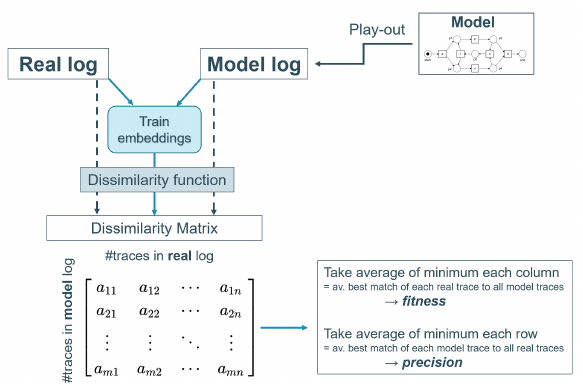
\includegraphics[width=.8\textwidth]{figures/structure}
	\caption{The general structure of the approach}
	\label{fig:structure}
\end{figure}


Three different techniques were outlined in the focus paper \cite{PBWe20}, all following a similar structure outlined in \cref{fig:structure}.
First, a model log is produced from the model by using appropriate replay semantics for the model.
Then, given these two logs, one real and one produced by replaying the model, it is possible to train the \emph{act2vec} \cite{KBWe18} embedding.
Based on these embeddings a dissimilarity function needs to be defined to compare different traces, however, the \emph{act2vec} embedding only yields distance measurements between activities and not between traces.
Here the differences between the three techniques come into play.
The first two, the Word Mover's Distance \cite{KSKW15} and Iterative Constrained Transfers, can directly utilize the distances between activities to determine a distance between two collections of activities.
The last one, \emph{trace2vec}, further needs to train a trace embedding based on activity embeddings, and can then perform direct comparisons in the trace embedding space.
All three methods however lead to a reasonable dissimilarity metric between traces.
Using one of these metrics a dissimilarity matrix can be built up describing the pairwise dissimilarities between the real log and the model log.

From here on we will assume that each row corresponds to a trace from the model log and each column corresponds to a trace from the real log, i.e. $a_{ij}$ is the dissimilarity of the $i$-th trace from the model log with the $j$-th trace of the real log.
As such, each column contains the dissimilarity of a trace in the real log with all traces from the model log, with the minimum of a column being the closest match in the model log.
A trace that can be closely replayed by the model, i.e. one that has a close match to a trace produced from the model, is a well-fitting one.
As such the column minimum corresponds to a fitness metric of the trace and thus the mean of all column minima is a fitness metric between log and log.
Conversely, each row contains all similarities between a trace in the model log and all traces in the real log.
A precise model should not allow for more traces than observed in the real log, so each model trace should have as close a match as possible in the real log for the model to be precise.
As such the row minimum corresponds to a precision metric for the trace in the model log and thus the mean of all row minima is a precision metric between the logs.

\subsection{act2vec}
The first two methods utilize \emph{act2vec} to train activity embeddings.
These activity embeddings then allow for the comparison of two traces by comparing their individual activities in the embedding space.
Every trace then constitutes a distribution over the embeddings of the activities contained in it, so given an appropriate distance metric for probability distributions such as the Earth Mover's Distance, it is possible to determine the distance (or conversely similarity) between two traces.
Note that many NLP algorithms use a so-called bag of words approach, where the order of words is disregarded.
Both the WMD and ICT take the same approach as a bag of words and treat a trace as a bag of activities.

\subsubsection{Word Mover's Distance}


\begin{algorithm}
	\caption{Word Mover's distance}\label{alg:wmd}
	\begin{algorithmic}
		\State $n:=$ vocabulary size
		\State $p_i,q_i := $ normalized count of activity $i$ in $p$ or $q$ respectively
		\State $c(i,j) :=$ Distance between embeddings of activity $i$ and $j$
		\Function{$F_{WMD}$}{$p,q,c$}
		\State distance $\gets$ $\min \sum_{i,j=1}^n T_{ij}c(i,j)$
		\State subject to:
		\State $\sum_{j=1}^{n}T_{ij}=p_i \forall i \in \{1,...,n\}$ \Comment{Outflow}
		\State $\sum_{i=1}^{n}T_{ij}=q_j \forall j \in \{1,...,n\}$ \Comment{Inflow}
		\State \Return distance
		\EndFunction
	\end{algorithmic}
\end{algorithm}
The Word Mover's Distance \cite{KSKW15} is a variant of the Earth Mover's Distance \cite{RTGu98} adapted for natural language processing.
This family of metrics has proved to be quite robust as well as accurate for a lot of embedding-based NLP tasks.
For this reason, it was chosen as an initial candidate for the distance function of an embedding-based conformance checking technique.
The Earth Mover's distance measures the distance between two probability distributions.
The informal interpretation of this is that there are two distributions, represented by piles of earth.
The distance between two distributions can be interpreted as the amount of work that needs to be done to transform one into the other.
Clearly, the work and thus the distance between two distributions depends on both the amount of earth on each of the piles and on the distance between piles.
Formally the EMD defines a distance metric for probability distributions over some vector space with a notion of distance.

This can be formulated as a linear program by formulating it as a min-cost-max-flow problem with two additional constraints. 
%The outflow constraint stating, that from each source-vertex no more can leave than actually present and an inflow constraint stating that now more can flow into each sink-pile no more can flow than being required.

In the case of embeddings and natural language processing this metric has also become known as the Word Mover's Distance.
Here the word embeddings represent the piles, i.e. the distance between two-word embeddings represents the "work" needed to transform one into the other, whereas collections of words, or more specifically their embeddings, such as sentences or even documents represent the probability distributions.

It should also be noted that the WMD does not take word order into account, which is reasonable for e.g. semantic classification of documents, but seems much more important in the case of business processes, where it seems intuitively important to avoid classifying $\langle a,b,c\rangle$ as being zero distance from a trace like $\langle c,b,a \rangle$.

\subsubsection{Iterative Constrained Transfers}
\begin{algorithm}
	\caption{ACT}\label{alg:act}
	\begin{algorithmic}
		\State $k:=$ number of edges considered per activity
		\State $p_i,q_i := $ normalized count of activity $i$ in $p$ or $q$ respectively
		\State $c(i,j) :=$ Distance between embeddings of activity $i$ and $j$
		\State $h_p,h_q :=$ amount of different activities in trace $p$ and trace $q$ 
		\Function{$F_{ICT}$}{$p,q,c,k$}
		\For{$i=1...h_p$}
		\State $s \gets \arg \min_k(c(i,[1,...,h_q]))$ \Comment{Find $k$ activities with the smallest cost}
		\While{$l < k$}
		\State $r \gets \min(p_i,q_{s(l)}))$ \Comment{Edge constraint}
		\State $p_i \gets p_i - r$ \Comment{Move weight}
		\State $t \gets t + rc(i,j)$ \Comment{Update cost}
		\State $l \gets l+1$
		\EndWhile
		\If{$p_i \neq 0$} \Comment{Move any remaining weight in $p_i$ to $q_{s(k)}$}
		\State $t \gets t + p_ic(i,s(k))$ \Comment{Move rest to $q_{s(k)}$}
		\EndIf
		\EndFor
		\State \Return $t$
		\EndFunction
	\end{algorithmic}
\end{algorithm}
The EMD and variants of it are very attractive since they are both very general and exhibit good accuracy for both search and classification.
A major drawback of such methods however is the cubic complexity in the size of the input distributions, which makes it infeasible for larger problems.
In the case of conformance checking the size of the input, distribution is determined by the number of activities in the log, for which good scalability is desired.
There are a number of techniques that aim to reduce the complexity of EMD-based approaches, that obtain an approximation of the EMD by relaxing some of the constraints.  
One example of such a method is the Relaxed Word Mover's distance which drops the second (inflow) constraint, thus greatly simplifying the solution.
While this makes it easier to calculate the solution, the RWMD only gives a lower bound on the WMD.
Another such method is the Iterative Constrained Transfers \cite{AtMi18} algorithm that has linear complexity in the size of the input distribution.
Instead of just dropping the inflow constraint it is instead replaced by an edge capacity constraint.
The main benefit of this is that it avoids the formulation as a linear program and is instead solvable using a much less powerful, but much quicker, direct algorithm.

Furthermore, there is also an approximation to the ICT called Approximate Computation of ICT (ACT), by limiting the number of iterations in said direct algorithm.
ICT and ACT agree in the limit, however, if the number of occurring activities is relatively low, even small numbers of iterations lead to sufficient results.
Only if there are some activities that occur significantly more often than others it is necessary to perform more iterations.

The ICT and ACT again provide a lower bound to the WMD, since it is not guaranteed that the inflow constraint is met, however, the ICT/ACT lower bound is higher than the RWMD lower bound due to the additional constraint that was introduced.

\subsection{trace2vec}
In contrast to the two previous approaches, which used activity embeddings, it is also possible to train trace embeddings.
The relationship between \emph{act2vec} and \emph{trace2vec} is analogous to the one between \emph{word2vec} and \emph{doc2vec}.
When using this method, every trace is embedded into a vector space and any distance metric that is deemed appropriate can be chosen.
In the paper, the cosine similarity \cref{eq:cosine} was chosen for its simplicity and the fact that it is bounded in the interval $[-1,1]$.
\begin{equation}
	\cos(x,  y) = \frac { x \cdot  y}{|| x|| \cdot || y||}
	\label{eq:cosine}
\end{equation}
This is much less computationally expensive than the previous two approaches which were complex distance metrics between two sets of embeddings.

\section{Experiments}
\label{sec:results}
To assess the performance of the three proposed embedding-based techniques the authors designed and performed three experiments.
These aimed to test and compare the scalability of the methods, whether noise deteriorates the results in an expected manner, and lastly to compare these techniques to established well-researched conformance checking techniques.

\subsection{Experimental Setup}
\begin{figure}
	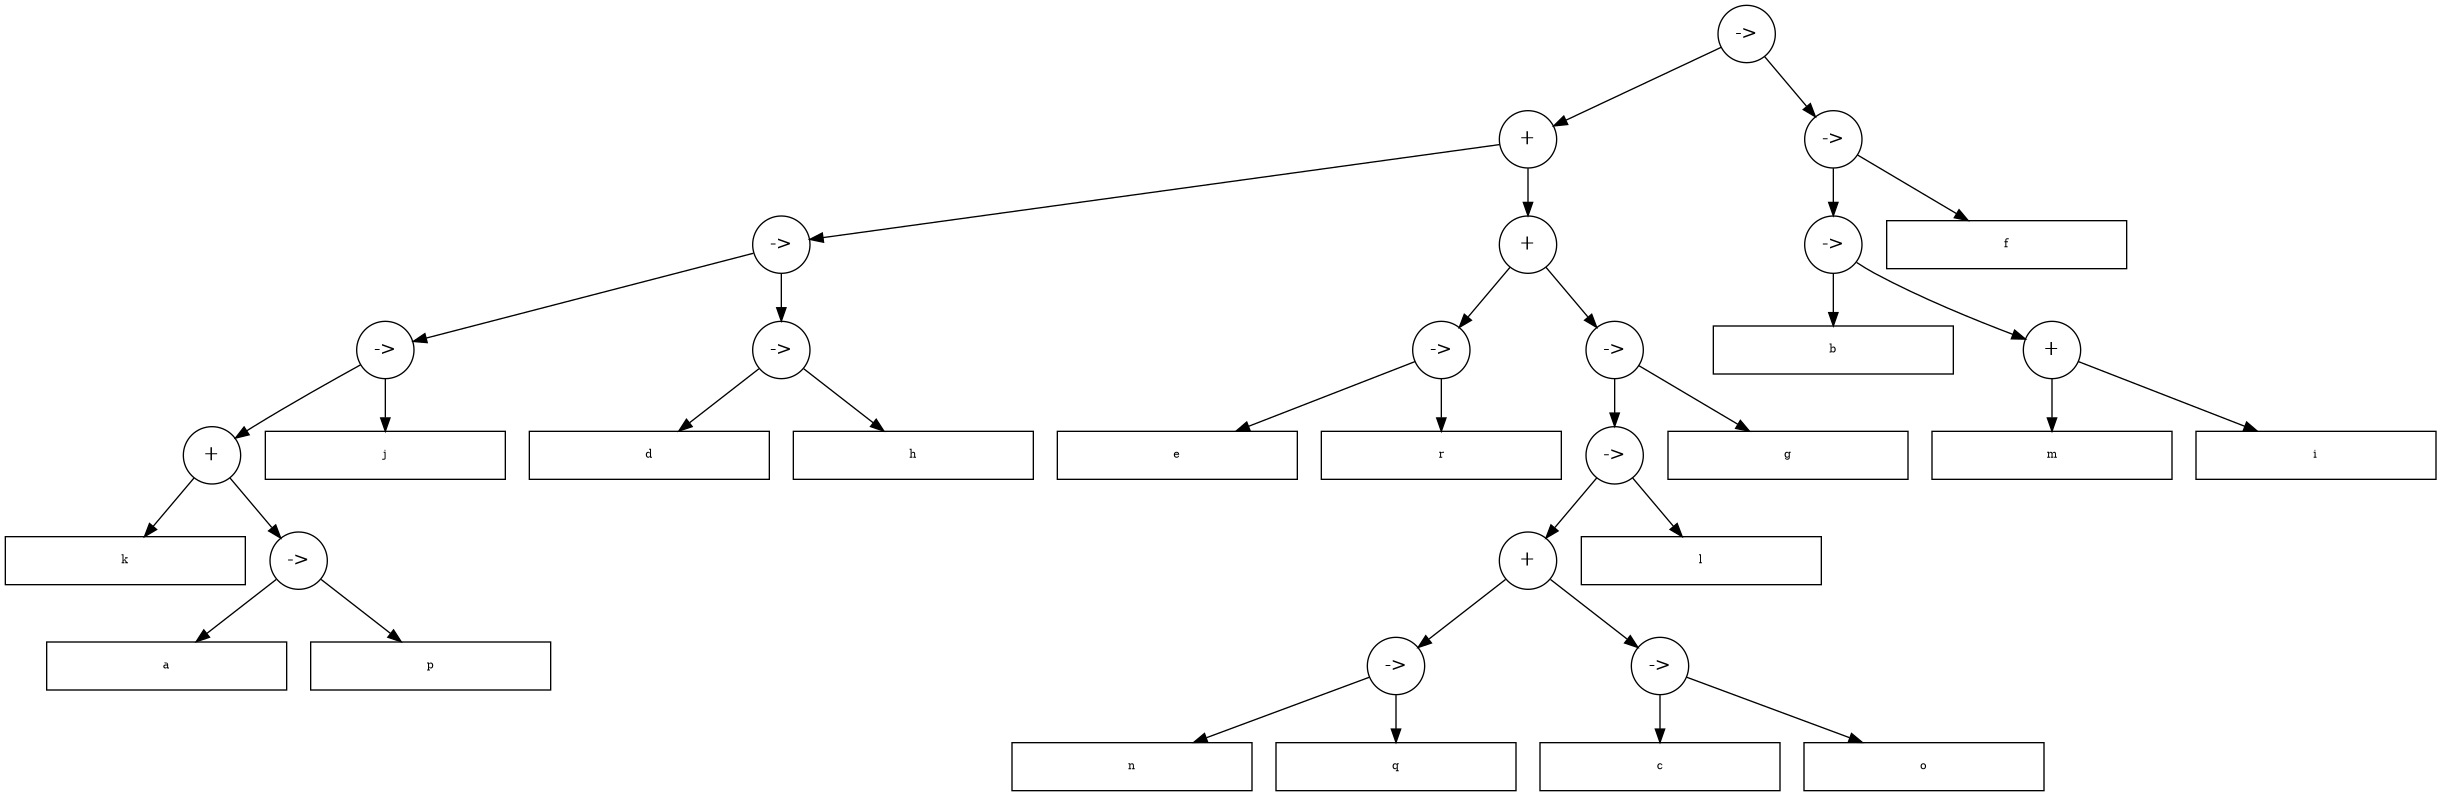
\includegraphics[width=1\textwidth]{figures/process-tree}
	\caption{A process tree generated by pm4py using parameters: Min 15, Mode 30, Max 45, sequence 0.75, parallel 0.25. }
	\label{fig:process-tree}
\end{figure}
%To evaluate the suitability of the method three sets of experiments were performed. 

All experiments utilized (the same) randomly generated process trees, that were constructed using the algorithms in the \emph{pm4py} library.
Three size configurations described by minimum number, the model, and the maximum number of visible activities were chosen: 5-10-15, 10-20-30, and 15-30-45.
Furthermore, four operator configurations were chosen described by the probability for randomly choosing each available operator.
These were in no particular order: Sequence: $0.75$, Parallel $0.25$, secondly Sequence: $0.75$, Choice $0.25$, thirdly Sequence: $0.5$, Parallel $0.25$, Choice $0.25$ and lastly $0.25$ for all (Sequence, Parallel, Choice and Loop) operators.
Both of these configurations were combined to generate a grid of $12$ process trees, with the hope that these cover a sufficient range of different behavior.
An example of such a random process tree is shown in \cref{fig:process-tree}
\footnote{Note that this tree is not the one used by the authors since they did not share their trees or logs, but one generated with the same parameters.}.


The first set of experiments focused on the scalability of the approach, especially since more traditional approaches do not scale well. This aspect is doubly important when talking about the Internet of Things, where the granularity of events is much easier controllable, which makes it possible to produce large amounts of event data with comparatively little effort.
Due to this scalability is an important factor for the IoT, since it is desired to process these large amounts of data.

The second set of experiments aimed to determine whether the method responded as expected when providing noisy logs.
These experiments were designed to verify the soundness of the approach.
This was done by generating logs from random process trees generated by pm4py, applying random noise on these logs, and determining the conformance between the noiseless and noisy logs.

Three different types of noise were used: replacing a random activity with another, swapping two random activities, and removing a random activity.
Then,  two noise experiments were performed.
In the first experiment, the percentage of traces that noise was applied to was varied between $10\%$ and $50\%$, but each noise type was applied at most once to each trace.
In the second experiment instead, the percentage of traces to which noise was applied was kept constant at $40\%$, but the number of activities to which noise was applied was varied.
Furthermore, the second experiment only utilized the replacement noise function  omitting the other two.

The expectation is that any reasonable conformance metric should deteriorate the more noise is added to the log.

The third and last set of experiments was designed to compare the performance of the proposed methods (WMD, ICT \& trace2vec) to existing established conformance metrics, namely alignments, behavioral fitness \cite{GMVB09} and ETC precision \cite{MuCa10}.
This was achieved by generating 1000 traces from a randomly generated process tree, to obtain an event log.
Then, a discovery algorithm was applied to this log to discover a model. Here, Alpha Miner, Inductive Miner infrequent (IMi) with noise levels 0 and 1, and the ILP Miner were selected as discovery algorithms.
Then fitness and precision between the discovered model and the real log were calculated using the previously mentioned algorithms as well as the method described in the paper.


\subsection{Scalability Experiment}
\begin{figure}
	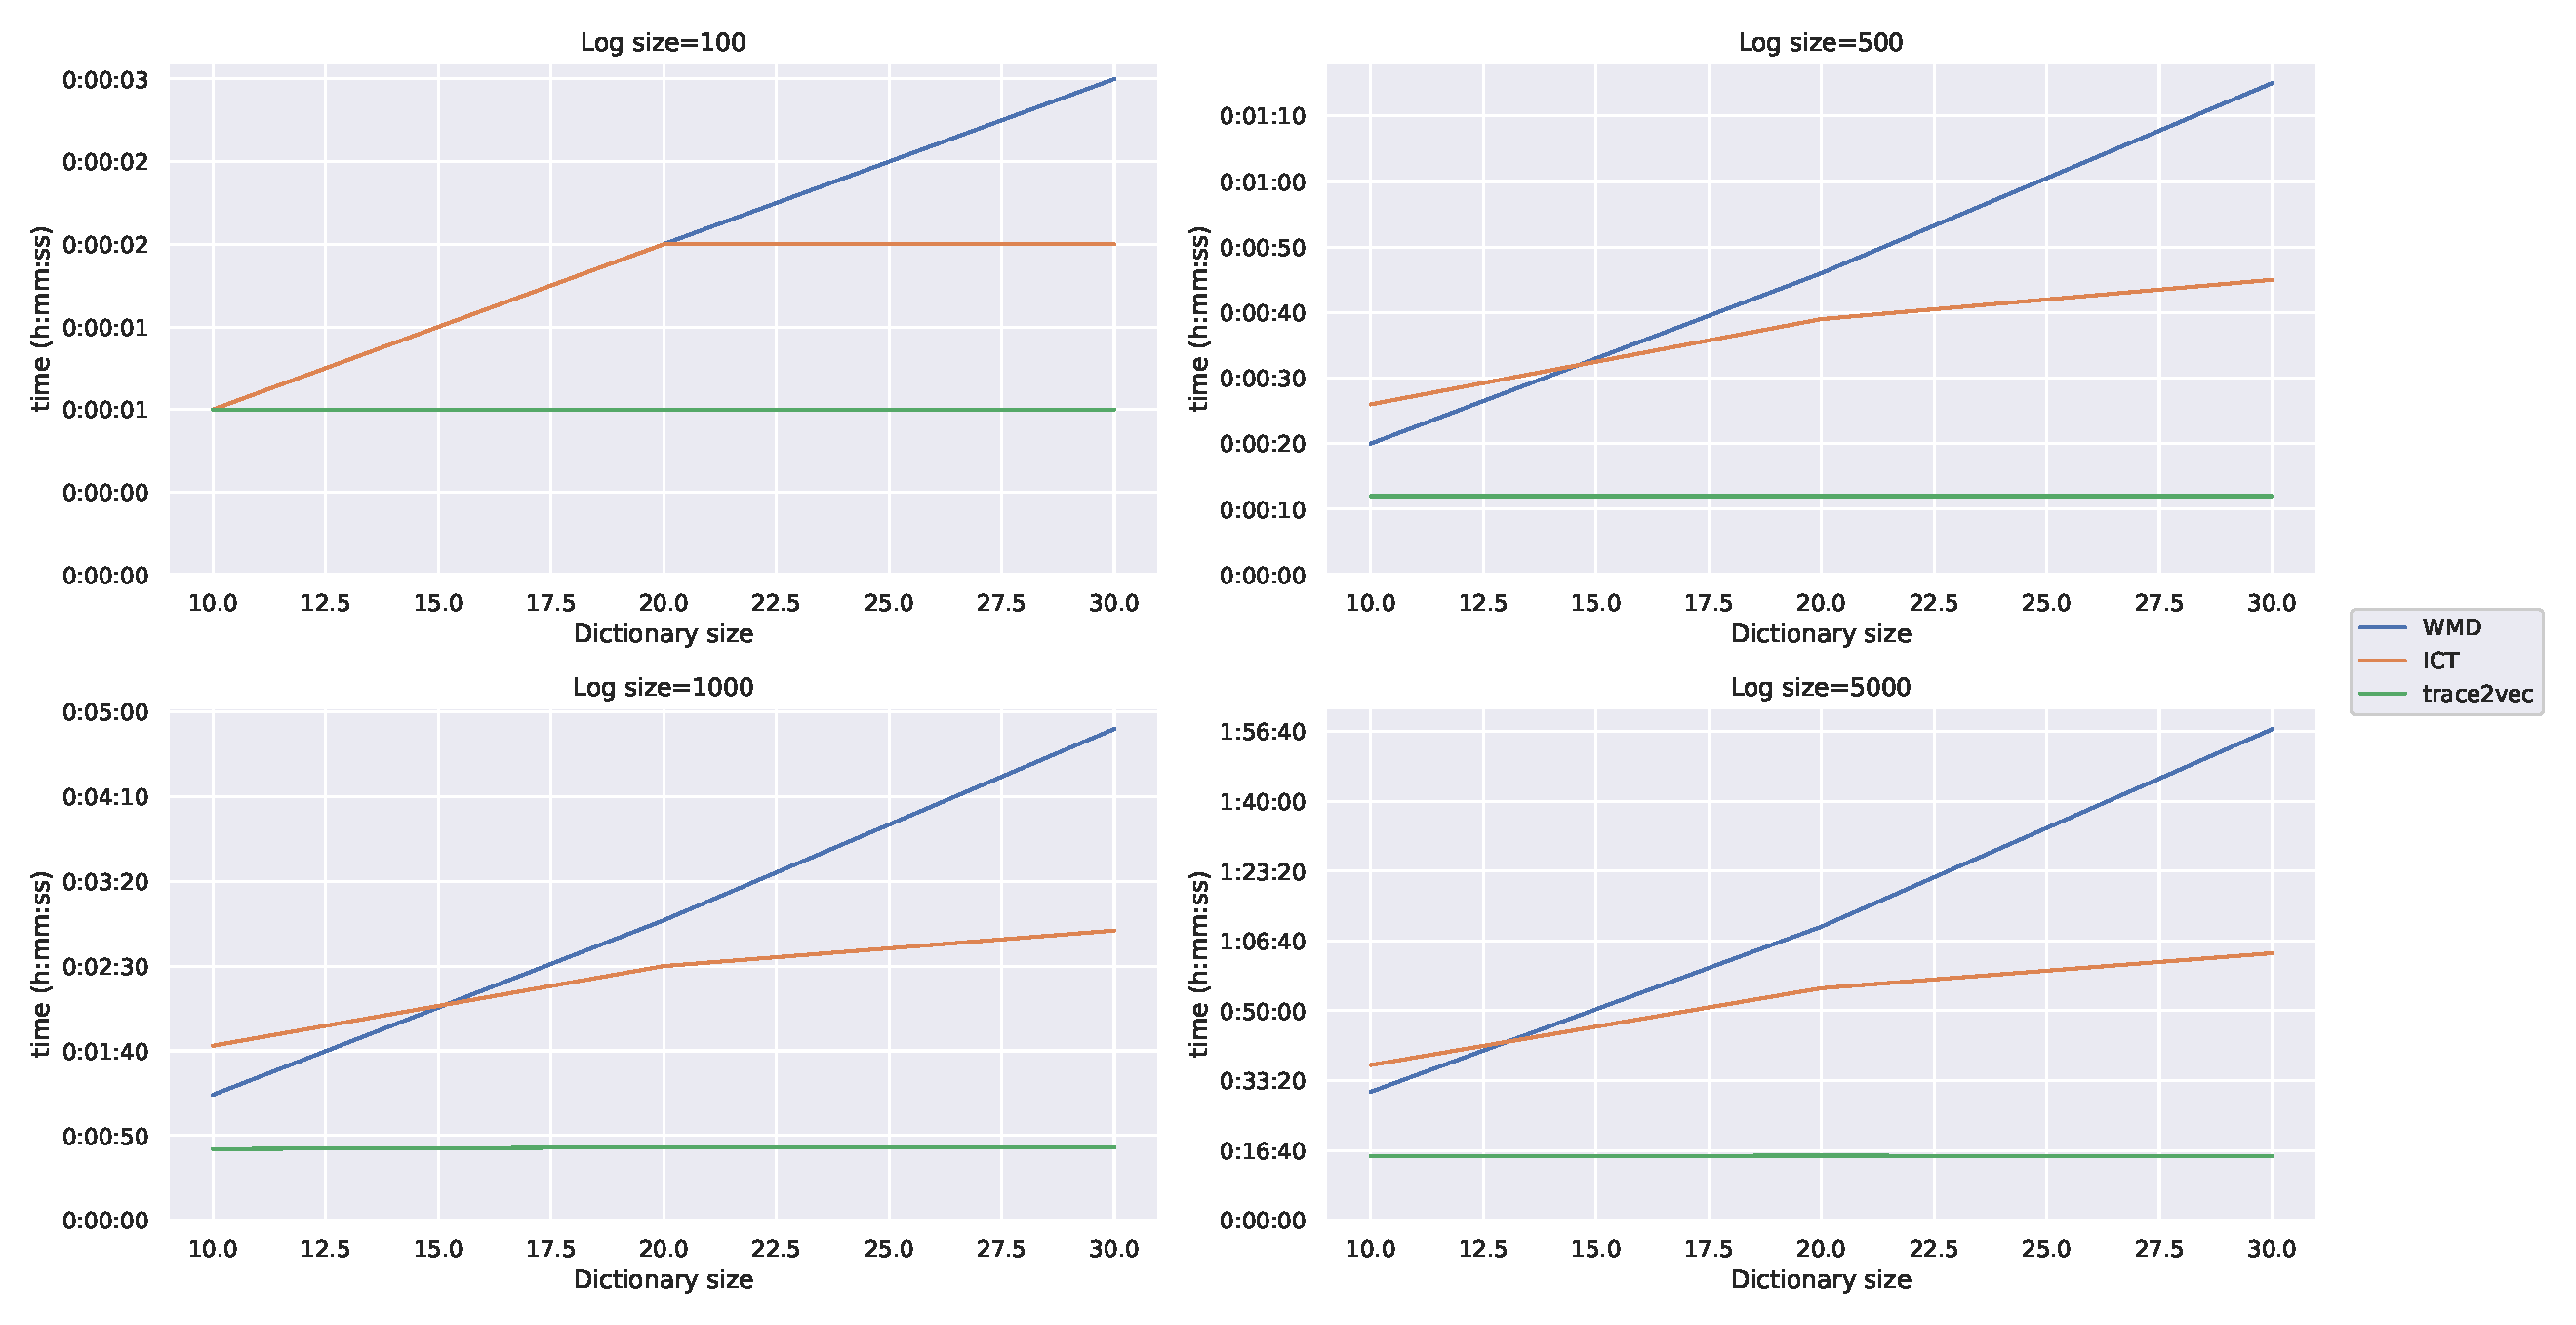
\includegraphics[width=1\textwidth]{figures/scaling}
	\caption{Runtimes for all three methods for varying sizes of logs and dictionaries. Data can be found in \cite{PBWe20} Table 2.}
	\label{fig:scalability}
\end{figure}
The first performed experiment aimed to assess the performance  of the three proposed methods.
The experiments were run on an Intel Core i7-9850h, a mid-range consumer CPU.
Experiments were run for all three methods for different sized logs and different sized dictionaries, for embedding-based conformance checking algorithms dictionary size is determined by the number of different activities in the log.
All experiments were performed in Python, however, the Word Mover's distance was calculated using pyemd, a Python wrapper to calculate the WMD/EMD with NumPy efficiency.
As such, when comparing ICT and WMD times, the efficiency difference between Python and C should be taken into account.

The resulting times are shown in \cref{fig:scalability}
\footnote{Note that when two logs of size $n$ are compared, $n^2$ comparisons are needed. This is the reason why the needed time scales quadratically with log size}.
Over all log sizes, a similar pattern is observable, with WMD and ICT behaving similarly and \emph{trace2vec} consistently outperforming the other two methods in all experiments.
For small dictionary sizes  (10) WMD does outperform ICT, however, that is likely due to the aforementioned efficiency differences between the implementations.
It is notable that despite these efficiency differences ICT already starts to outperform WMD for dictionary sizes of 20.
For dictionaries of size 30, this gap grows even larger.
Here ICT is finished after roughly half the time needed by the WMD approach.
These experiments seem to suggest that ICT scales much better with larger dictionary sizes.
Especially when considering that the current implementation is still unoptimized ICT could very well serve as a more efficient alternative to WMD, especially when working with complex logs.
It should also be noted that the relative run time difference between both methods slightly scale in the ICT's favor, starting out at $\frac{45}{75}=0.6$ for a log of size 500 and improving to $\frac{3824}{7032}\approx 0.54$ for logs of size 5000.

Lastly, the \emph{trace2vec} method substantially outperforms both the other methods, since only the cosine similarity, a simple mathematical formula needs to be evaluated at run time.
This comes with the additional overhead of training trace embeddings, however, according to the authors training that "does not take a long time" but they don't include statistics in that regard.
The \emph{trace2vec} method has the additional benefit of not being dependent on the activities during run time, since traces are directly compared in the trace embedding space, which means that the size of the dictionary is irrelevant for this approach, making it even more attractive for processes with large numbers of activities than the ICT.

\subsection{Noise experiment}
\begin{figure}
	\centering
	\begin{subfigure}[b]{0.49\textwidth}
		\centering
		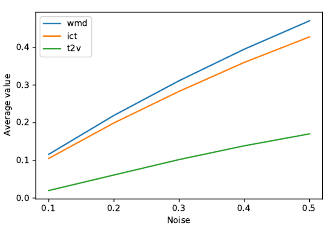
\includegraphics[width=\textwidth]{figures/noise-first}
		\caption{Average of first noise experiment (Varying trace percentage) }
		\label{fig:noise-first}
	\end{subfigure}
	\hfill
	\begin{subfigure}[b]{0.49\textwidth}
		\centering
		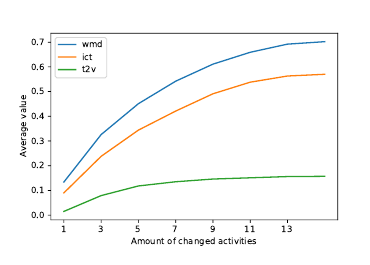
\includegraphics[width=\textwidth]{figures/noise-second}
		\caption{Average of second noise experiment (Varying amount of noise applied to trace)}
		\label{fig:noise-second}
	\end{subfigure}
\caption{Results from noise experiment (from \cite{PBWe20} Fig. 4 \& 5). Raw data can be found in \cite{PBWe20} Table 4}
\label{fig:noise}
\end{figure}
The second experiment aimed to determine how the algorithms behaved when different amounts of noise were introduced on the logs.
The expectation is that higher levels of noise further deteriorate fitness and precision. 
However since the defined similarity notion is not very intuitive it is important to verify, whether the algorithms are well-behaved, i.e. if their results match up with the intuitive expectation we have for conformance.
%However since the used methods are somewhat involved and since it can be hard to exactly tell what a system is doing for a lot of learning-based methods, whether the algorithms are well-behaved or not should be verified.

Fo all noise experiment three random tree using the configurations mentioned above were created, from which the "noiseless" logs were produced.
Then two different kind of noise were applied to these logs, and the average distance between traces in the "noiseless" and "noisy" variant was compared.
These results can be found in \cref{fig:noise}.

The first noise experiment in which the number of noisy traces was varied seems to confirm the expectation.
In all the trees, the distance smoothly increased with larger amounts of noise added, there were neither cases where the dissimilarity would go down again with more noise nor any significant unexpected patterns like jumps or plateauing around certain points.
The average of all the values from the first noise experiment is shown in \cref{fig:noise-first}.
Here it is also clearly visible that the dissimilarity gain slows down for larger levels of noise, however, that is perfectly expected. 

The second noise experiment also seems to back up the soundness of the approach, where the dissimilarity again increased, the more activities were replaced.
The results from the second noise experiment can be seen in \cref{fig:noise-second}.

It should be noted that for both experiments the absolute values for WMD and ICT are not comparable to \emph{trace2vec}, since these are on different scales.

\subsection{Discovery Experiment}
\begin{figure}
	\centering
	\begin{subfigure}[b]{0.49\textwidth}
		\centering
		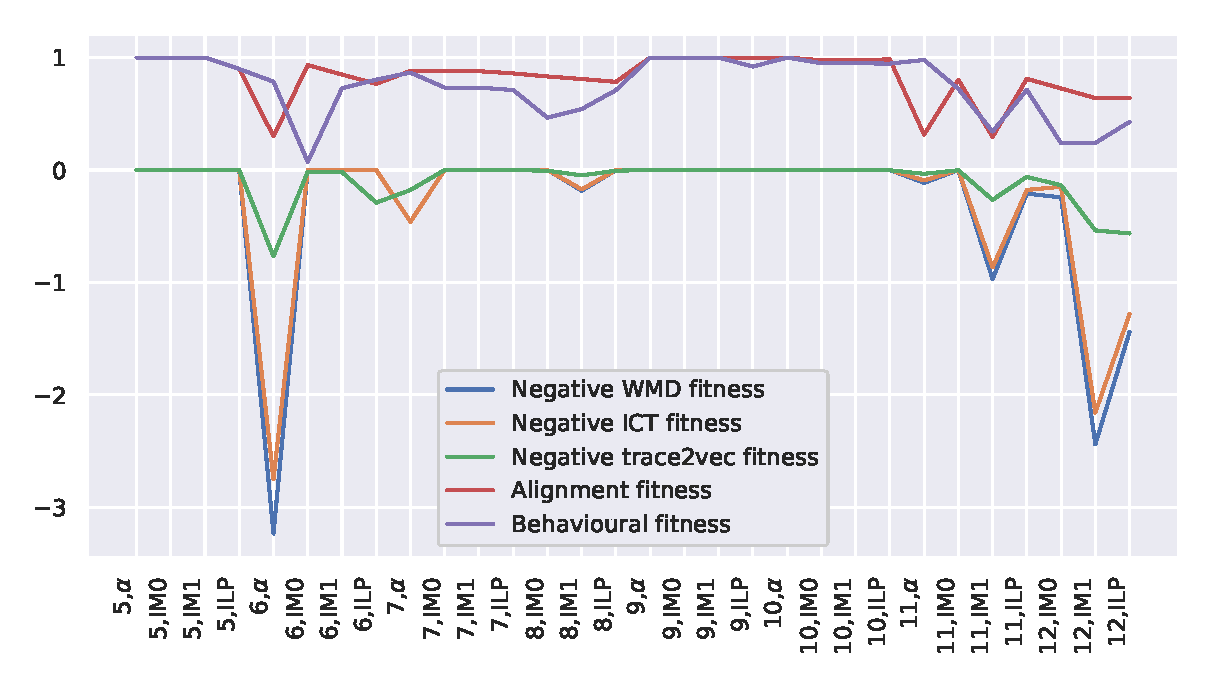
\includegraphics[width=\textwidth]{figures/fitness}
		\caption{Fitness}
		\label{fig:fitness}
	\end{subfigure}
	\hfill
	\begin{subfigure}[b]{0.49\textwidth}
		\centering
		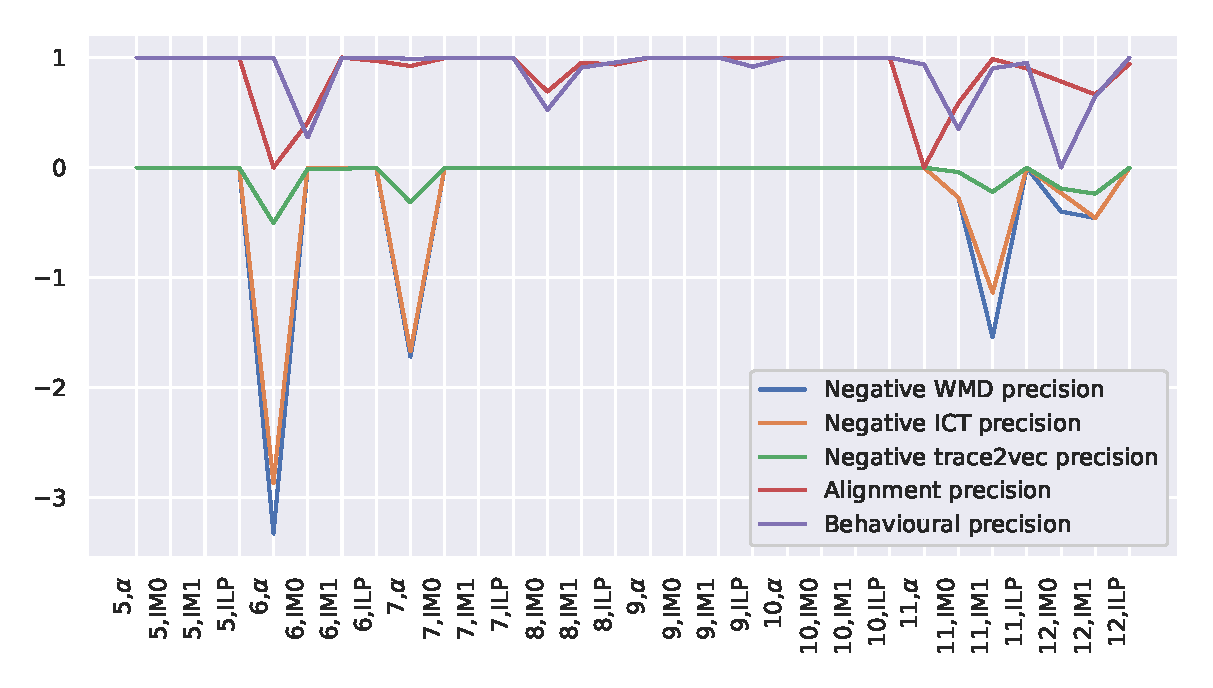
\includegraphics[width=\textwidth]{figures/precision}
		\caption{Precision}
		\label{fig:precision}
	\end{subfigure}
	\caption{Fitness and Precision for different tree, discovery technique pairings for the three proposed techniques as well as the two verification techniques. 
		Note that values are shown for WMD,ICT and \emph{trace2vec} are mirrored along x, since they are not proper metrics and larger values means worse fitness/precision. 
		This way all results move in the same direction for better/worse values.
		Raw data can be found in \cite{PBWe20} Table 5.}
	\label{fig:discovery}
\end{figure}

The purpose of the last experiment was the comparison of the three proposed techniques to establish conformance checking algorithms.
The results of this experiment can be found in \cref{fig:discovery}.
The results from the discovery experiment seem to suggest that all three methods are able to capture a notion of conformance.
Especially when the model is of high quality both the proposed and validation conformance checking techniques often agree on a perfect score.
However, it should be noted that there are quite a few instances where all three proposed methods assign perfect fitness or precision despite the others producing imperfect scores.
This is worrying since one of the most basic requirements for a good conformance checking technique is not assigning perfect scores to models that are able to replay fewer or more traces than in the log.
It is unclear whether that is due to the unoptimized nature of the methods, it could be the case that the methods are not sensitive enough, which could be fixed by varying the parameters, or due to the limited size of the model logs, which were limited to 1000 traces, which puts an upper limit on the amount of behavior that the embeddings are able to observe.

Yet when models deteriorate there is a tendency for all measurements to move together.
At the current point, only a qualitative analysis for imperfect models is possible since the values determined by WMD, ICT and \emph{trace2vec} are not proper metrics since they do not fall into the $0,1$ range.
As such it is hard to interpret what a non-optimal value actually means, and therefore the data does not allow for a quantitative comparison  at this point.
The results that were obtained however suggest that these methods could be a useful alternative to established techniques and that further research into them is warranted.

It is of course also important to point out that the validation techniques should not be seen as perfect normative techniques, since both of these also significantly disagree for some models. 

\subsection{Reproduction of Experiments}
The authors published some \href{https://github.com/jaripeeperkorn/Conformance-checking-using-activity-and-trace-embeddings}{source code} accompanying the paper.
To verify their results as well as possibly perform some additional experiments it seemed appropriate to look at said code and try to reproduce their results as well as possible.
After some initial technical difficulties, since very specific package versions were needed, their code was successfully run.
They provide three separate Python scripts for their implementations of the  WMD, ICT and \emph{trace2vec} methods.

Aside from that they also provide Jupyter notebooks for their experiments, however sadly these do not run the whole experiment, instead, they only perform the experiment for one parameter combination.
To reproduce their noise experiment it is thus necessary to manually run the corresponding notebook twelve times, once for each parameter combination, manually note down the results of each run, and merge them manually at the end.
This was deemed to be out of scope for this paper.
Additionally, the discovery experiment only determined the fitness and precision of the WMD, ICT, and \emph{trace2vec} methods and not the reference methods, so it is unclear at this point how the fitness and precision values for the reference methods were determined.
Overall it can be said that the results from the paper are at least partially reproducible, and the provided implementation gives a good pointer into how the methods were set up in detail, but running the experiments and collecting the results requires more effort than should be necessary.

Lastly, it was considered to design and run another experiment here to evaluate performance and scaling differences between the embedding based approaches and reference approaches like alignments, behavioral fitness, and ETC precision, as this is one of the main selling points especially in the IoT and the authors sadly did not include an experiment to that effect.
In light of the complications with the existing experiments and the fact that no evaluation of the reference metrics was included in their code, this idea was deemed out of scope for this paper.

\section{Discussion}
\label{sec:discussion}
\subsection{Future Work}
Peeperkorn et al. obtained promising first results for a novel embedding-based approach towards conformance checking.
Yet as the focus was mainly on the introduction and development of a prototype for such an approach there are some natural limitations.
Arguably the biggest limitation were the logs used for the experimental validation.
All used logs were completely synthetic, generated from random process trees.
It is unclear how well the 12 trees used for this resemble real processes and whether these tree configurations are sufficiently representative for the variation exhibited in real life trees\footnote{12 tree configurations were used, 3 sizes and 4 different probability distributions for operations, how strong these vary should be investigated}.
As such it should be a priority to test the proposed methods on real logs, possibly popular benchmark cases, and also to systematically broaden the parameters for random process tree generation to cover more different classes.


It is also a  prerequisite for further research and possible usage of such methods to convert the distance metrics obtained into proper conformance metrics, especially by restricting values to the interval $[0,1]$.
When that is done further quantitative comparisons between the updated methods and established conformance checking techniques should be performed.
Furthermore, the algorithms used have several parameters which were set as seemingly reasonable standard values.
A thorough investigation into the effect of these parameters should follow since it can not be known whether similar defaults should be used in conformance checking  as in classical NLP problems.
Special attention should be placed on those cases for which the NLP techniques produced perfect values, whereas the others did not.
The methods should be tested with completely perfect and completely imperfect models regarding fitness and precision, as well as nearly perfect and nearly imperfect models to verify that the methods are able to correctly classify both ends of the model spectrum and not misclassify nearly optimal models as perfect.

Apart from that two of the metrics proposed -- WMD and ICT -- do not take the order of words/activities into account.
This is due to the fact that for a lot of NLP problems order is of lesser importance and tasks like document keyword detection can treat a document as an order-less bag of words.
At least from an intuitive understanding of conformance checking, the order of activities is integrally important, and it should at least be investigated if there are significant differences between ordered and orderless approaches with regard to conformance checking.
The authors themselves suggest considering the use of $n$-grams instead of 1-grams, since their application seems more feasible in business processes as compared to classical NLP.

Lastly, the paper should be understood as a successful first use of NLP-related algorithms for the task of conformance checking.
The use of embeddings is often the easiest method in such approaches, but it is entirely possible that more advanced NLP algorithms may give even better results.
As such further research into the applicability of a variety of other methods could be fruitful.
The authors especially mention $n$-grams, Embeddings from Language Models, Global Vectors for Word Representation, and Recurrent Neural Networks.


\subsection{Internet of Things}
When analyzing such an approach in the context of the Internet of Things, there are three main facets that need to be considered.
Due to the fact that the Internet of Things itself, as well as its architectures, are very heterogeneous, it will always be possible to find networks where one of the following limitations or requirements does not hold to some extent, however generally speaking the following should be the main considerations when trying to adapt a process management technique to the Internet of Things.
First, the Internet of Things generates a lot of data, and the amount of potential data that can be generated is enormous.
This means high performance, for things like real-time analysis, is a major goal.
The second consideration should be that the Internet of Things is very "online", in the sense that events are constantly produced and thus analysis, such as conformance checking, during process execution is a highly desired property of any technique. 

\subsubsection{Performance}
An important question that was not yet properly addressed is whether this method offers benefits in the use case of the internet of things and how well it would be adaptable to such an environment.
The first important thing to note in that regard is performance.
Sadly the authors did not include a performance measure for the baseline methods but it should be noted that there was one case where alignments did not produce a result in a reasonable time frame. 
However, it is well known that alignments are a rather inefficient technique due to the inherent non-determinism and complex search structures needed to find an optimal alignment.
As such it should be pointed out that any performance efficient technique that rivals alignments in expressive power, is desired in normal process mining, while being doubly important in any environment where computing power is much more limited and where data needs to be processed in real-time.
Furthermore, embeddings provide a way to move computations out of the conformance calculation into preliminary calculations, namely determining the embedding function.
While the embeddings were trained separately and independently for each tree in the focus paper, a good embedding function for a process's activities and/or traces could theoretically be shared in the Internet of Things.
This is attractive since it further decreases the amount of work needed to evaluate a dissimilarity, and, as can be seen at the \emph{trace2vec} case, generally exhibits much better scaling properties.
Separating the conformance checking algorithm into a (more) efficient and well-scaling evaluation part and a less efficient but shareable training part could make such algorithms much more desirable in use-cases with many activities, long traces, and/or high-performance requirements, such as real-time evaluation.
\subsubsection{Online/Streaming algorithms}
An online conformance checking technique based on alignments is presented in \cite{ZBK*19}.
Online conformance checking generally has two problems. Not underestimating the conformance of running traces, as running traces are missing events necessary for completion, while not overestimating the conformance of terminated traces, without explicit knowledge of termination.

A naïve way to perform conformance checking analysis of the prefixes using the techniques outlined above is to simply add all prefixes of traces in the model log  to the model log.
This approach essentially replicates the prefix-conformance technique presented \cite{ZBK*19} for any model-log to real-log technique.
The basic approach there was to relax one of the restrictions, namely that the end marking of an alignment had to be a final marking, to consider all traces whose end marking can reach the final marking, i.e. that there exists some remainder execution that completes the trace.
Given a large enough sampling, this is equivalent to enumerating all prefixes of the replay.
While this approach would give decent estimations for any incomplete traces such an approach runs into several problems.
The first is that the explosion of the model log greatly increases the number of (dis)similarities that need to be calculated, which degrades performance.
Secondly, as for all online conformance checking algorithms that don't assume explicit knowledge of termination, this will greatly overestimate the conformance of many non-fitting traces, especially since the fitness of a trace is a minimum of all distances between itself and model traces, it is very sensitive to the sudden inclusion of a lot of new model traces.
Precision would be less affected by such a change since the percentage of incomplete traces in the real log is assumed to be relatively small.

However, more complicated techniques are also imaginable.
Both WMD and ICT seem rather problematic approaches, when it comes to online conformance checking as both require normalization over activities, so even a prefect prefix like $\langle a,b\rangle$ of $\langle a,b,c\rangle$ would be encoded as $(0.5,0.5,0)$ and $(0.33,0.33,0.33)$ respectively.
This means that through the modeling approach prefix relationships are already substantially degraded.
It is possible that there are subset-like variants of the WMD, however, I am not aware of any.

The \emph{trace2vec} method could be more interesting since it gives a framework to directly compare traces.
If we look at any trace we would assume that the longer a prefix we take and determine the embedding of, the more similar it is to the trace itself, i.e. it converges in some sense to the embedding of the complete trace.
An improvement on the naïve method above could be to just check all prefixes of the $k$ nearest neighbors to any trace.

Overall it should be noted that online conformance checking is a difficult problem, but that there are certainly possibilities for solutions using the proposed techniques, especially considering their novelty there has been less research on how they could be adapted in an online setting, and how such adaptions perform in reality.
But even beyond that, there are many potential interesting use cases for embedding-based methods in an online method.
For example, the use case of predicting the next activity, while outside the bounds of conformance checking, maps very cleanly to word prediction tasks, when using embeddings, so there are certainly very interesting topics in applying embeddings to not only conformance checking  but other process mining tasks as well.

%
% ---- Bibliography ----
%
% BibTeX users should specify bibliography style 'splncs04'.
% References will then be sorted and formatted in the correct style.
%
\bibliographystyle{template/splncs04}
\bibliography{literature/bibliography}
%
\end{document}
